\documentclass{article}
\usepackage[utf8]{inputenc}
\usepackage{graphicx}
\usepackage{url}
\title{\Huge{CS296 Project - Group 19\\}}
\author{\Large{Abhinav Gupta} (120050029)\\\Large{Anant Gupta} (120050029)\\\Large{Stephan Biastoch} (13V051004)\\ }
\date{\Large{10 April 2014}}

\begin{document}

\maketitle
\pagebreak
\section{Introduction}
The project is a working model of the Glock 23 pistol built using the Box2D\cite{box2d} physics engine.
\\
\\
Glock 23 is a semi-automatic pistol which includes firing of the bullet, extraction and ejection of the casing and reloading of the pistol on pressing the trigger.
\\
\\
Here's an image of the same\cite{genitron}.
\\
\begin{figure}[hbtp]
\centering
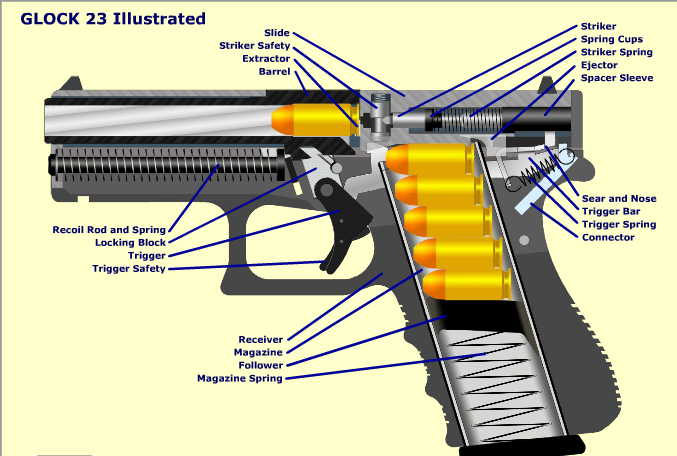
\includegraphics[scale=0.3]{glock.png}
\caption{\texttt{Glock 23 Illustrated}}
\end{figure}
\pagebreak
\section{Design}
Here's the Lab 1 design of the gun.
\\
\begin{figure}[hbtp]
\centering
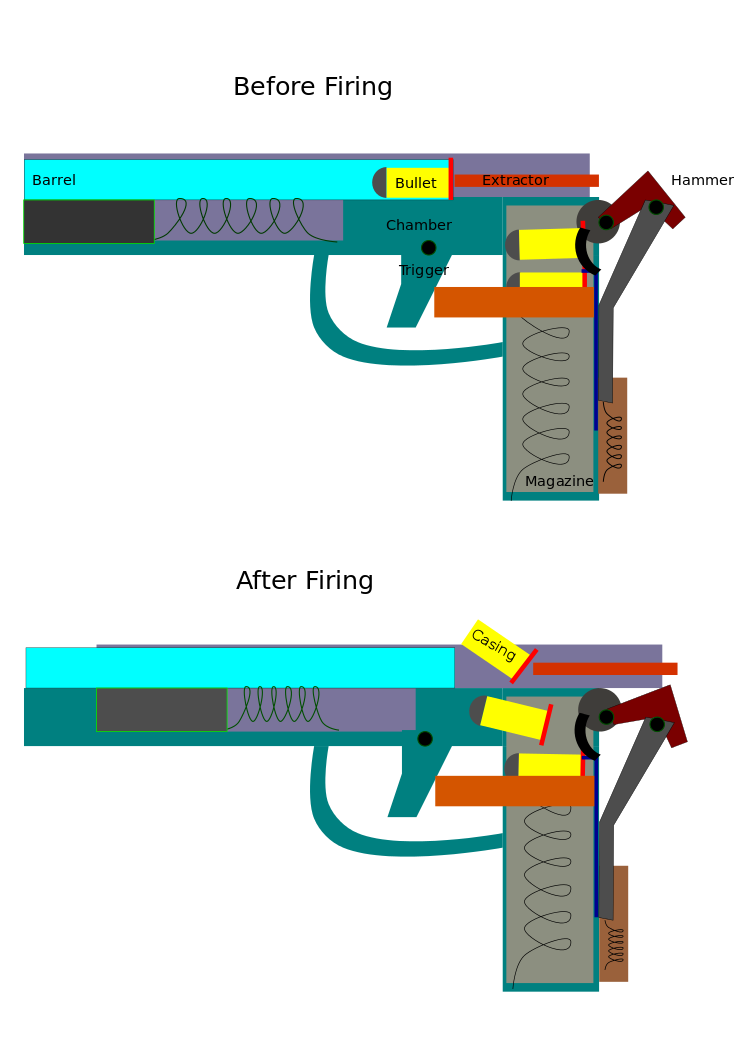
\includegraphics[scale=0.3]{gun.png}
\caption{\texttt{Inkscape Design}}
\end{figure}
\\
This design has been more or less implemented in the project. Some movements, which were beyond the scope of Box2D have been artificially created using impulses.
\pagebreak
\section{Working}
This section describes the working of the gun in Box2D.
\subsection{Striker Assembly}
When the trigger is pressed, the striker spring gets compressed. When the contact between the connector and the striker assembly is lost, the spring expands making the striker hit the bullet casing.

\subsection{Barrel and Slide}
In reality, when the striker hits the casing a small explosion is created causing the bullet to move forward and the barrel and slide to recoil. However, for the project the explosion is simulated by giving impulse to the bullet and the barrel.

\subsection{Magazine}
The magazine contains a compressed spring on which the bullets are placed. When the gun cocks, there is an open space and the spring gets slightly released pushing a bullet into the barrel.
\subsection{The Code}
\begin{itemize}
\item The code creates the various objects in the dominos.cpp file.
\item The collisions are detected in the beginContact function of the b2ContactListener class by setting and checking the UserData variable of the bodies\cite{iforce}.
\item The impulses mentioned in the previous section are provided in this contact callback function.
\item We let physics take care of everything else.
\end{itemize}
\subsection{Stages}
Here are the various stages of the simulation.
\\
\begin{figure}[hbtp]
\centering
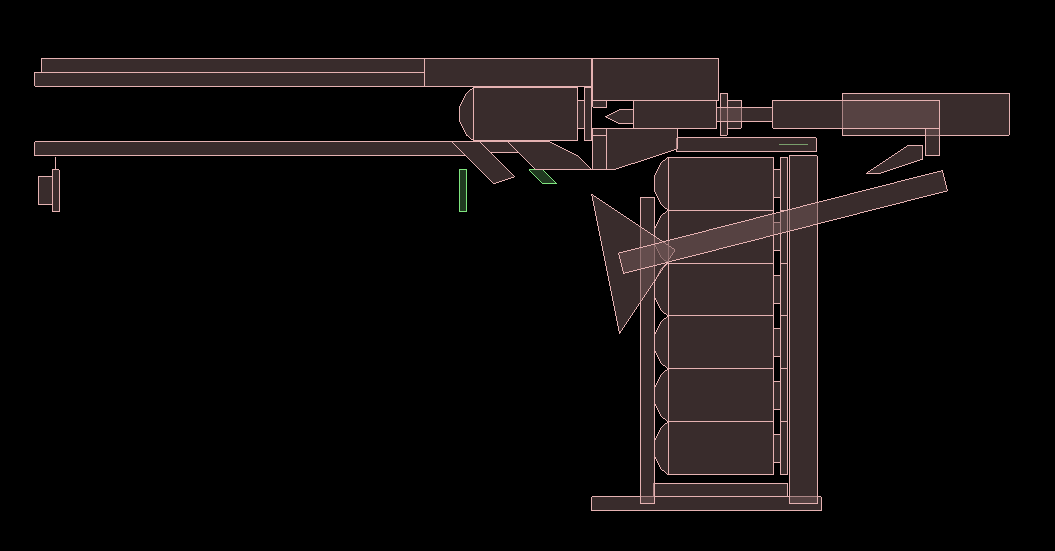
\includegraphics[scale=0.3]{before_firing.png}
\caption{\texttt{The gun before firing}}
\end{figure}
\\
\\
\begin{figure}[hbtp]
\centering
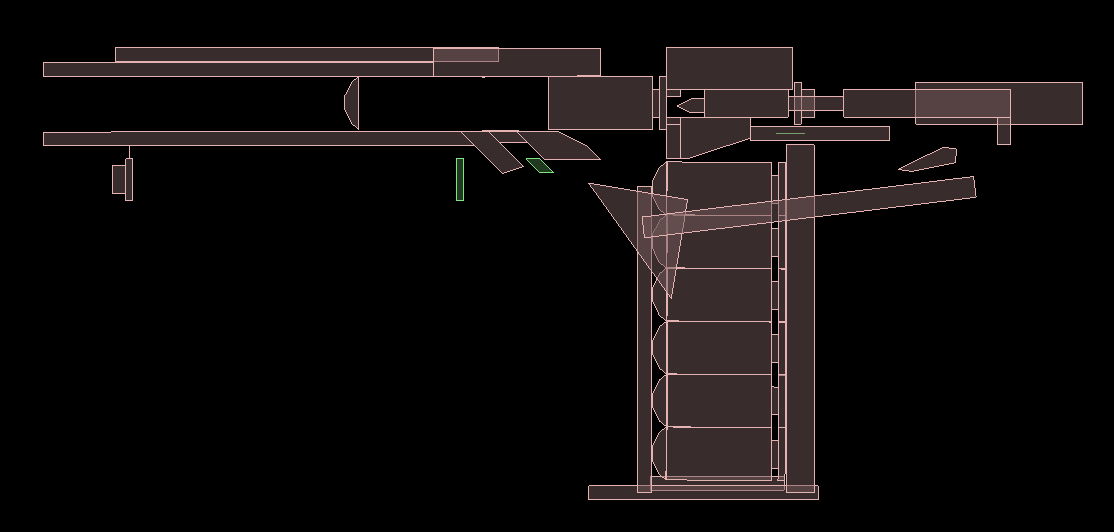
\includegraphics[scale=0.3]{shoot.png}
\caption{\texttt{The gun after being tirggered}}
\end{figure}
\\
\\
\begin{figure}[hbtp]
\centering
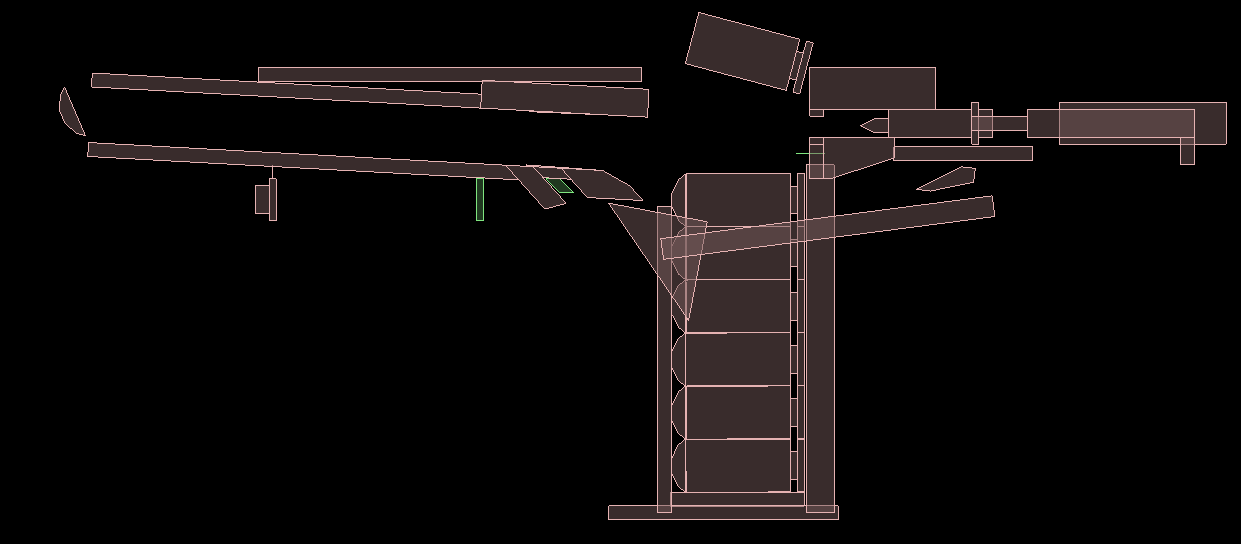
\includegraphics[scale=0.3]{ejection.png}
\caption{\texttt{Ejection of the Casing}}
\end{figure}
\\
\\
\begin{figure}[hbtp]
\centering
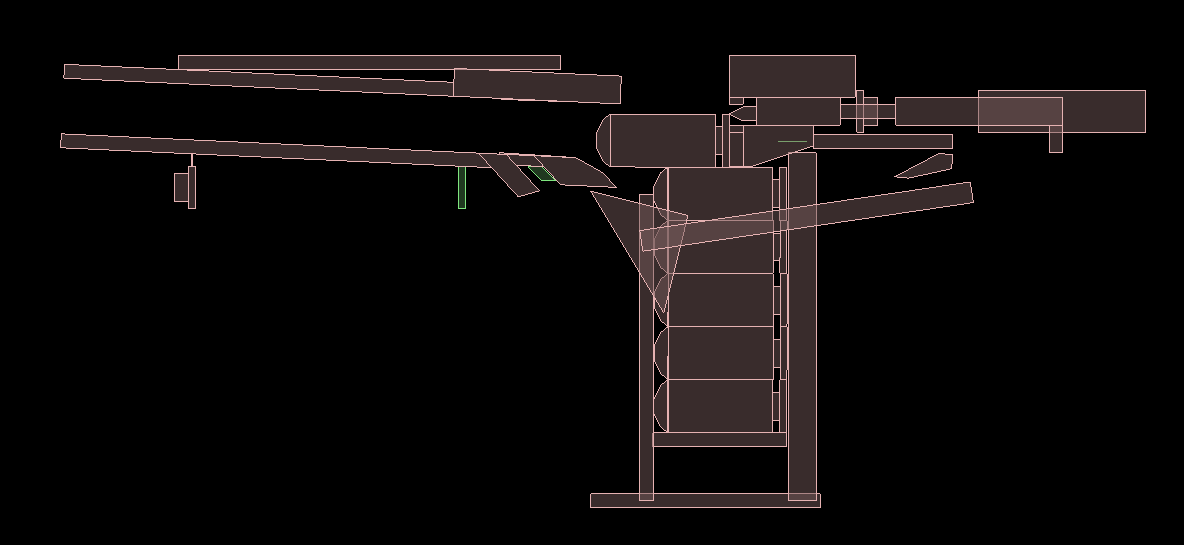
\includegraphics[scale=0.3]{reload.png}
\caption{\texttt{Reloading of the barrel}}
\end{figure}
\\
\\
\begin{figure}[hbtp]
\centering
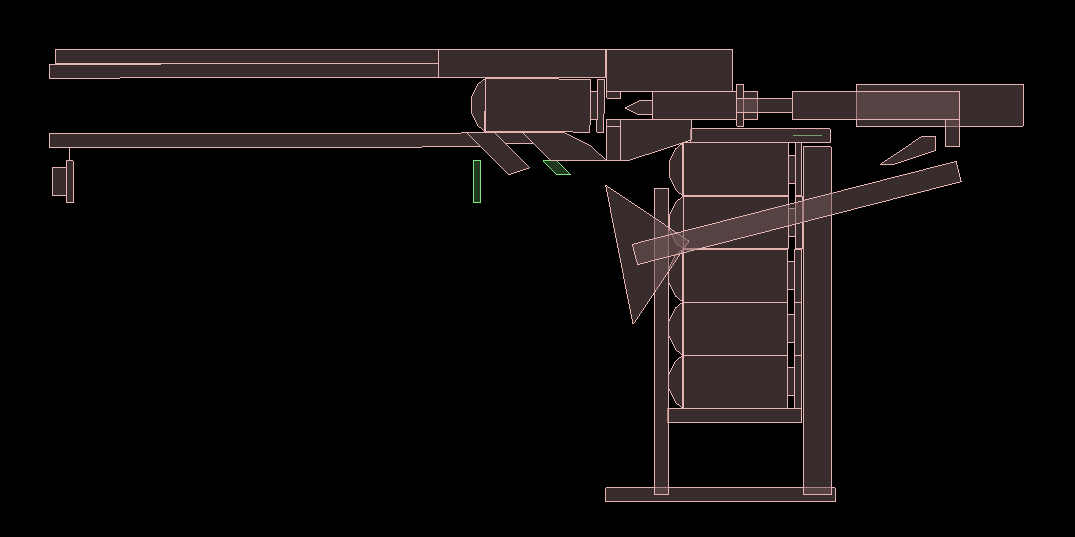
\includegraphics[scale=0.3]{after_firing.png}
\caption{\texttt{The gun after firing}}
\end{figure}
\\
\pagebreak
\pagebreak
\section{Timing and Profiling}
\subsection{Timing}
The following are the graphs for the step times for different number of iterations (from 1 to 100).
\\
\begin{figure}[hbtp]
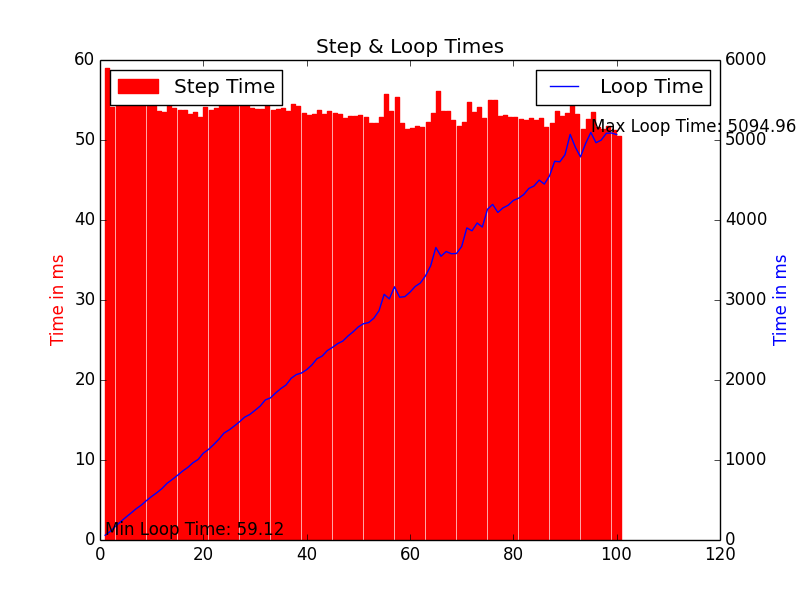
\includegraphics[scale=0.3]{plot1.png}
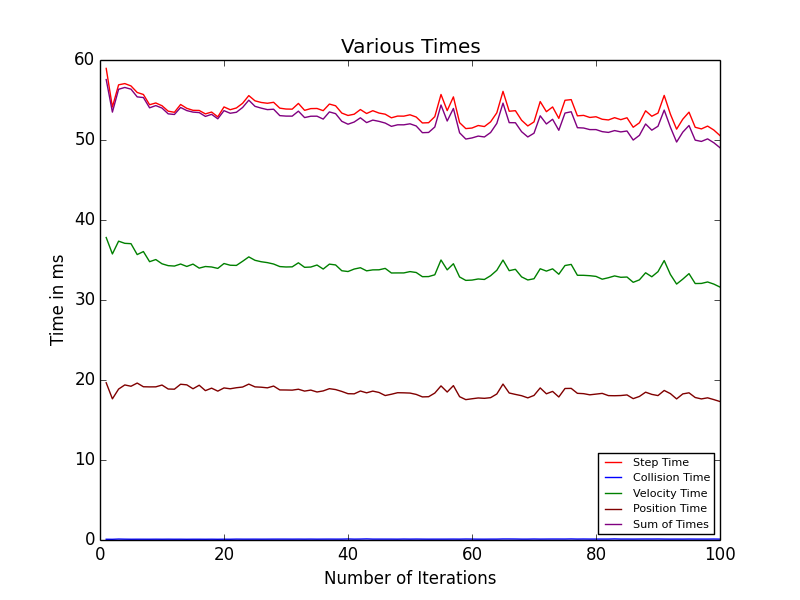
\includegraphics[scale=0.3]{plot2.png}
\caption{\texttt{Plots}}
\end{figure}
\\
It can be seen in the plot that the step times remain roughly the same on increasing the number of iterations which is to be expected because each step is a very intensive process due to the complex arrangement of the gun. This causes the calculation time to dominate any overhead time, which would have resulted in higher average step times for a lower number of iterations.
\\
\\
Furthermore, the collision times are negligible because the physics involves a large number of complex position and velocity calculations, thereby outweighing the time required for collisions.
\pagebreak
\subsection{Profiling}
Here is what the profile data looks like:
\\
\begin{figure}[hbtp]
\centering
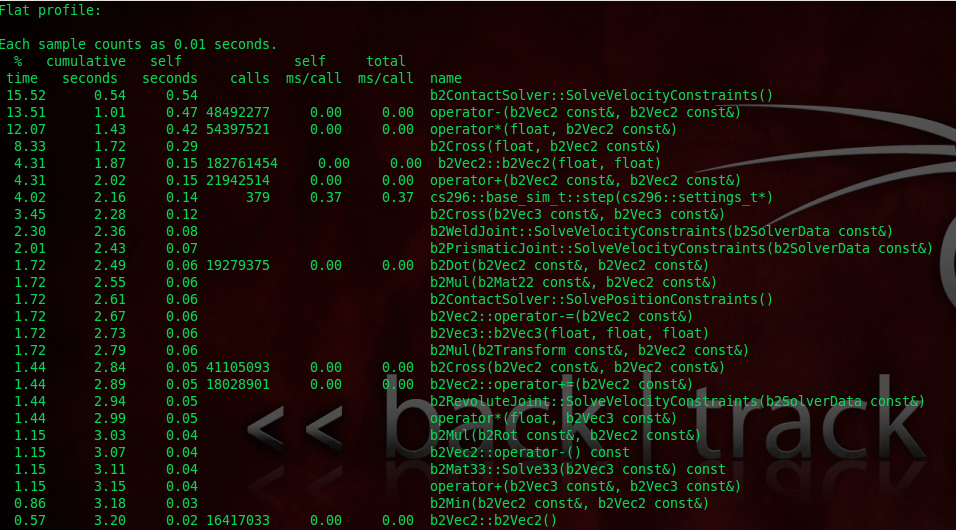
\includegraphics[scale=0.3]{profile.png}
\caption{\texttt{Profile Data}}
\end{figure}
\\
The call graph can be found under callgraph.png (not included in the report due to absurd dimensions).
\\
\\
A portion of the call graph looks like this:
\\
\begin{figure}[hbtp]
\centering
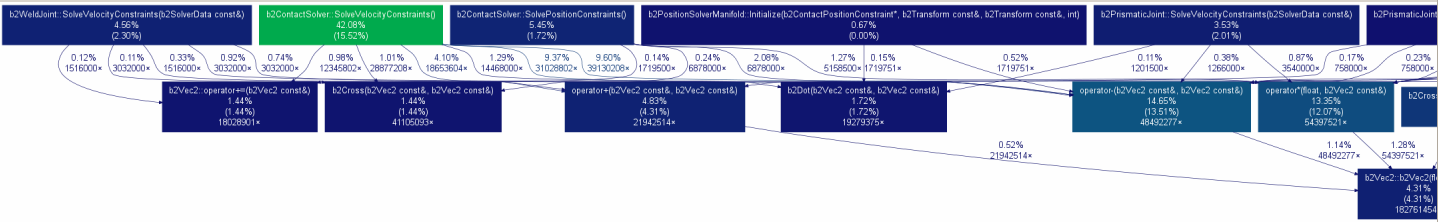
\includegraphics[scale=0.3]{callgraph_part.png}
\caption{\texttt{Call Graph}}
\end{figure}
\\
Since most of the time consuming functions are Box2D implementations, little can be done to optimize the simulation.
\\
\\
However, it may be possible to design the gun in such a fashion that is more stable and involves lesser moving parts.
\pagebreak
\bibliographystyle{te}
\bibliography{references}
\end{document}
